\documentclass[lang=cn,11pt,a4paper,cite=authornum]{paper}

\title{大数据技术基础 实验四 \\ 实验报告}
\author{毛子恒 \\ 2019211397}
\institute{北京邮电大学\ 计算机学院}

\date{\zhtoday}

% 本文档命令
\nocite{*}

\begin{document}

\maketitle

\section{概述}

\subsection{实验目的}

\begin{enumerate}
    \item 了解服务器配置的过程;
    \item 熟悉使用Scala编写Spark程序;
    \item 了解Spark RDD的工作原理;
    \item 掌握在Spark集群上运行程序的方法。
    \item 掌握Hive安装部署运行的方式。
    \item 掌握Spark读取Hive方式。
\end{enumerate}

\subsection{实验步骤}

\begin{enumerate}
    \item Hadoop集群环境测试;
    \item Spark集群搭建;
    \item Scala程序编写。
    \item 程序打包与运行;
    \item 安装Hive;
    \item Hive 建库并导入数据;
    \item 修改并运行程序。
\end{enumerate}

\section{实验结果及分析}

\paragraph{Spark集群搭建}

Spark集群部署结果如\figref{fig:spark1}和\figref{fig:spark2}。

\begin{figure}[!htb]
    \centering
    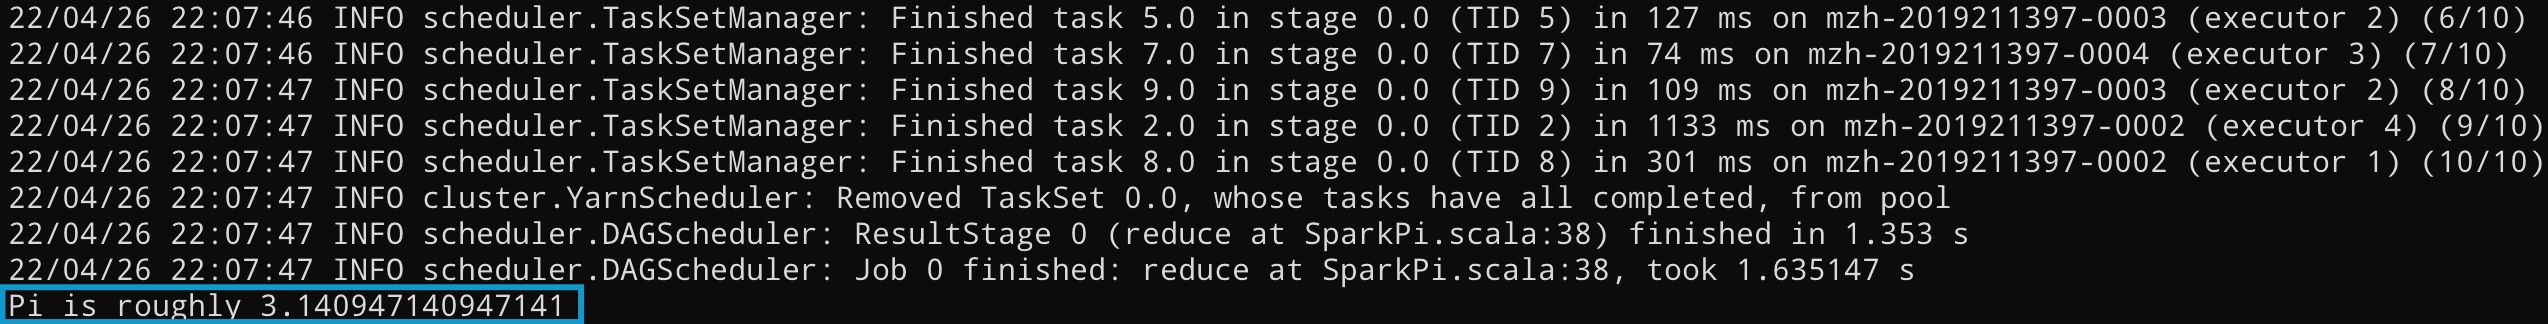
\includegraphics[width=\textwidth]{./images/spark1.jpg}
    \caption{Spark集群部署结果\label{fig:spark1}}
\end{figure}

\begin{figure}[!htb]
    \centering
    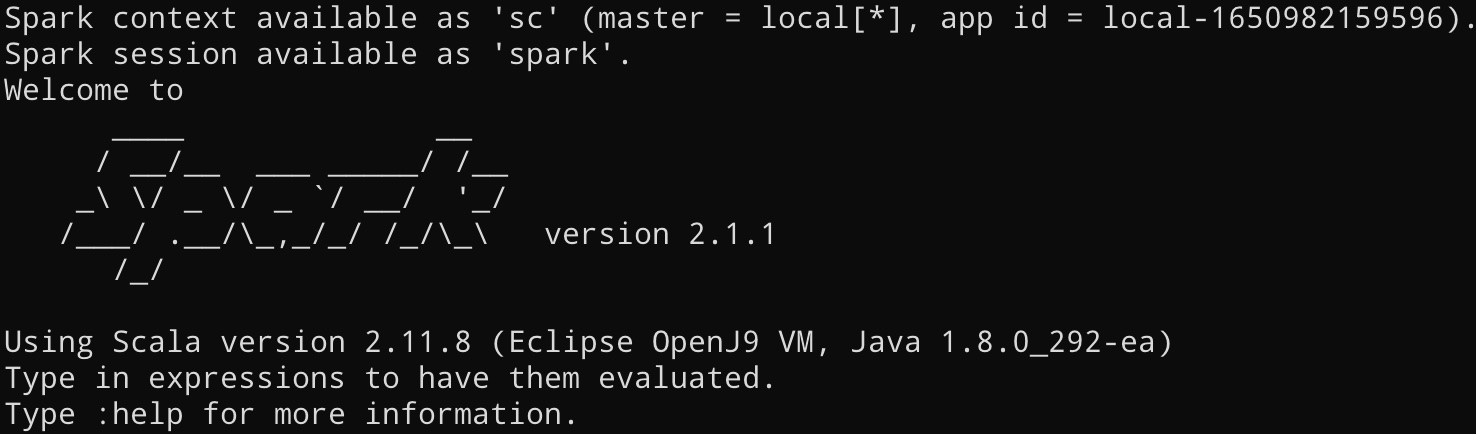
\includegraphics[width=\textwidth]{./images/spark2.jpg}
    \caption{Spark版本信息\label{fig:spark2}}
\end{figure}

使用Spark框架计算速度更快,得到$\pi$的精度更高。

\paragraph{程序打包和运行}

编写程序如\figref{fig:code1}。

\begin{figure}[!htb]
    \centering
    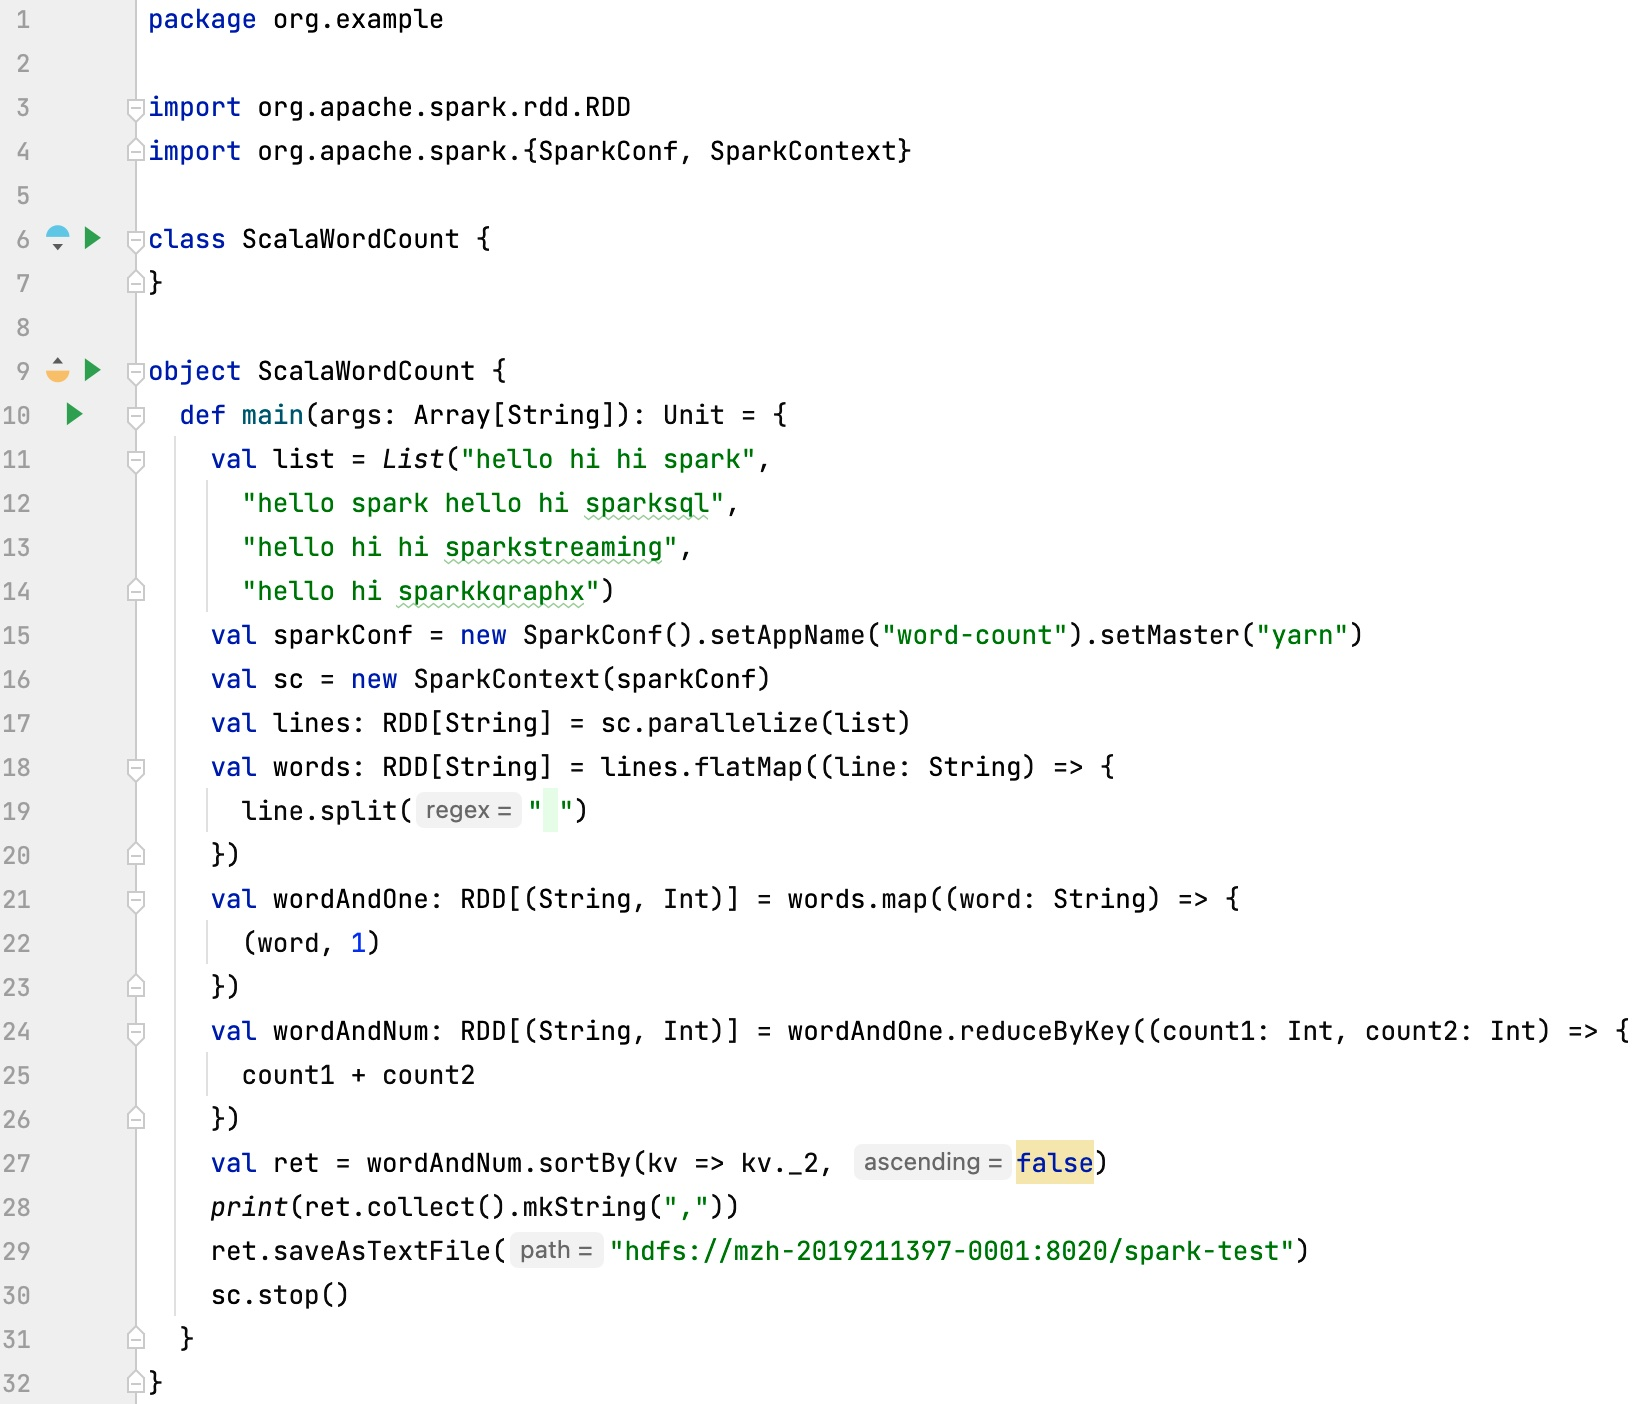
\includegraphics[width=0.7\textwidth]{./images/code1.jpg}
    \caption{wordcount程序\label{fig:code1}}
\end{figure}

程序中创建了一个字符串列表,配置一个Spark任务,之后利用\mintinline{text}{parallelize}方法生成RDD lines,其元素为字符串语句。将每个lines按照空格切分成单词,生成\mintinline{text}{words}RDD对象。再以单词为键,1为值建立键值对\mintinline{text}{wordAndOne}RDD对象,调用\mintinline{text}{reduceByKey}方法实现聚合操作,得到\mintinline{text}{wordAndNum}RDD对象。最后将\mintinline{text}{wordAndNum}按照值降序排序,打印到控制台。

将程序打包,上传到服务器运行,程序运行的结果如\figref{fig:res1}、\figref{fig:res2}和\figref{fig:res3}。

可见Spark统计了每个单词出现的次数,将结果保存到\mintinline{text}{/spark-test/}文件夹中。

\begin{figure}[!htb]
    \centering
    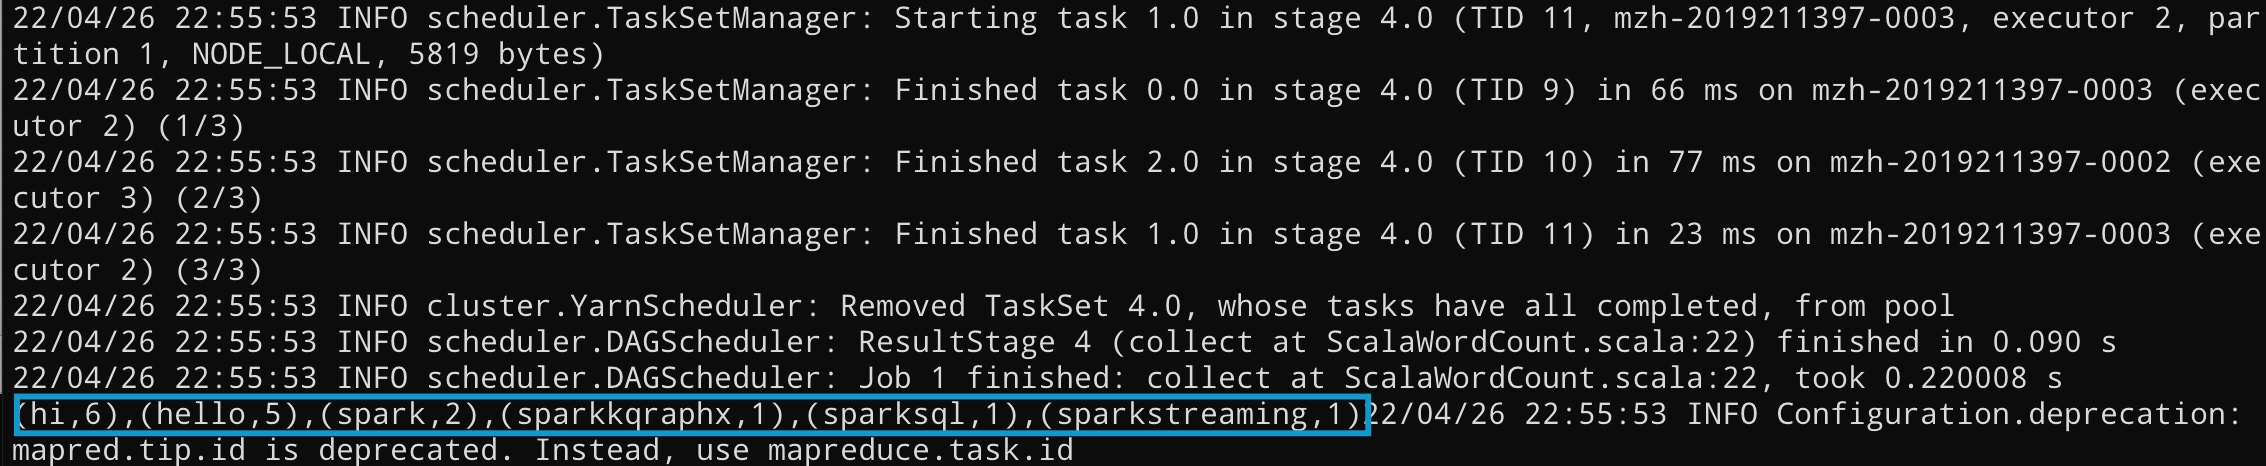
\includegraphics[width=\textwidth]{./images/res1.jpg}
    \caption{运行结果\label{fig:res1}}
\end{figure}

\begin{figure}[!htb]
    \centering
    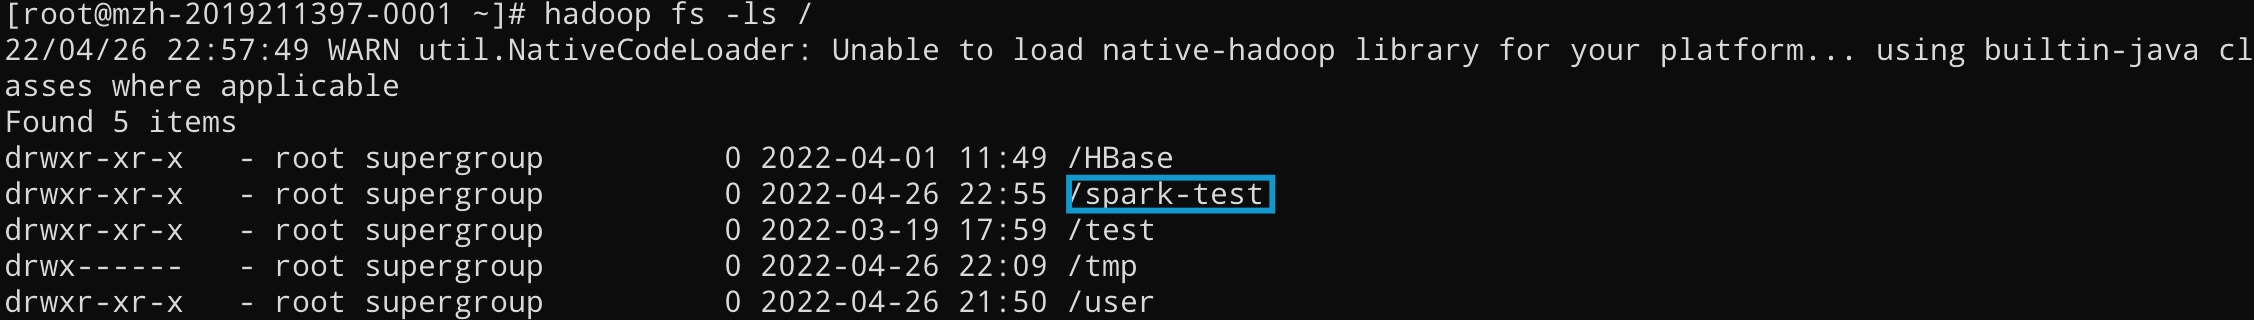
\includegraphics[width=\textwidth]{./images/res2.jpg}
    \caption{运行结果\label{fig:res2}}
\end{figure}

\begin{figure}[!htb]
    \centering
    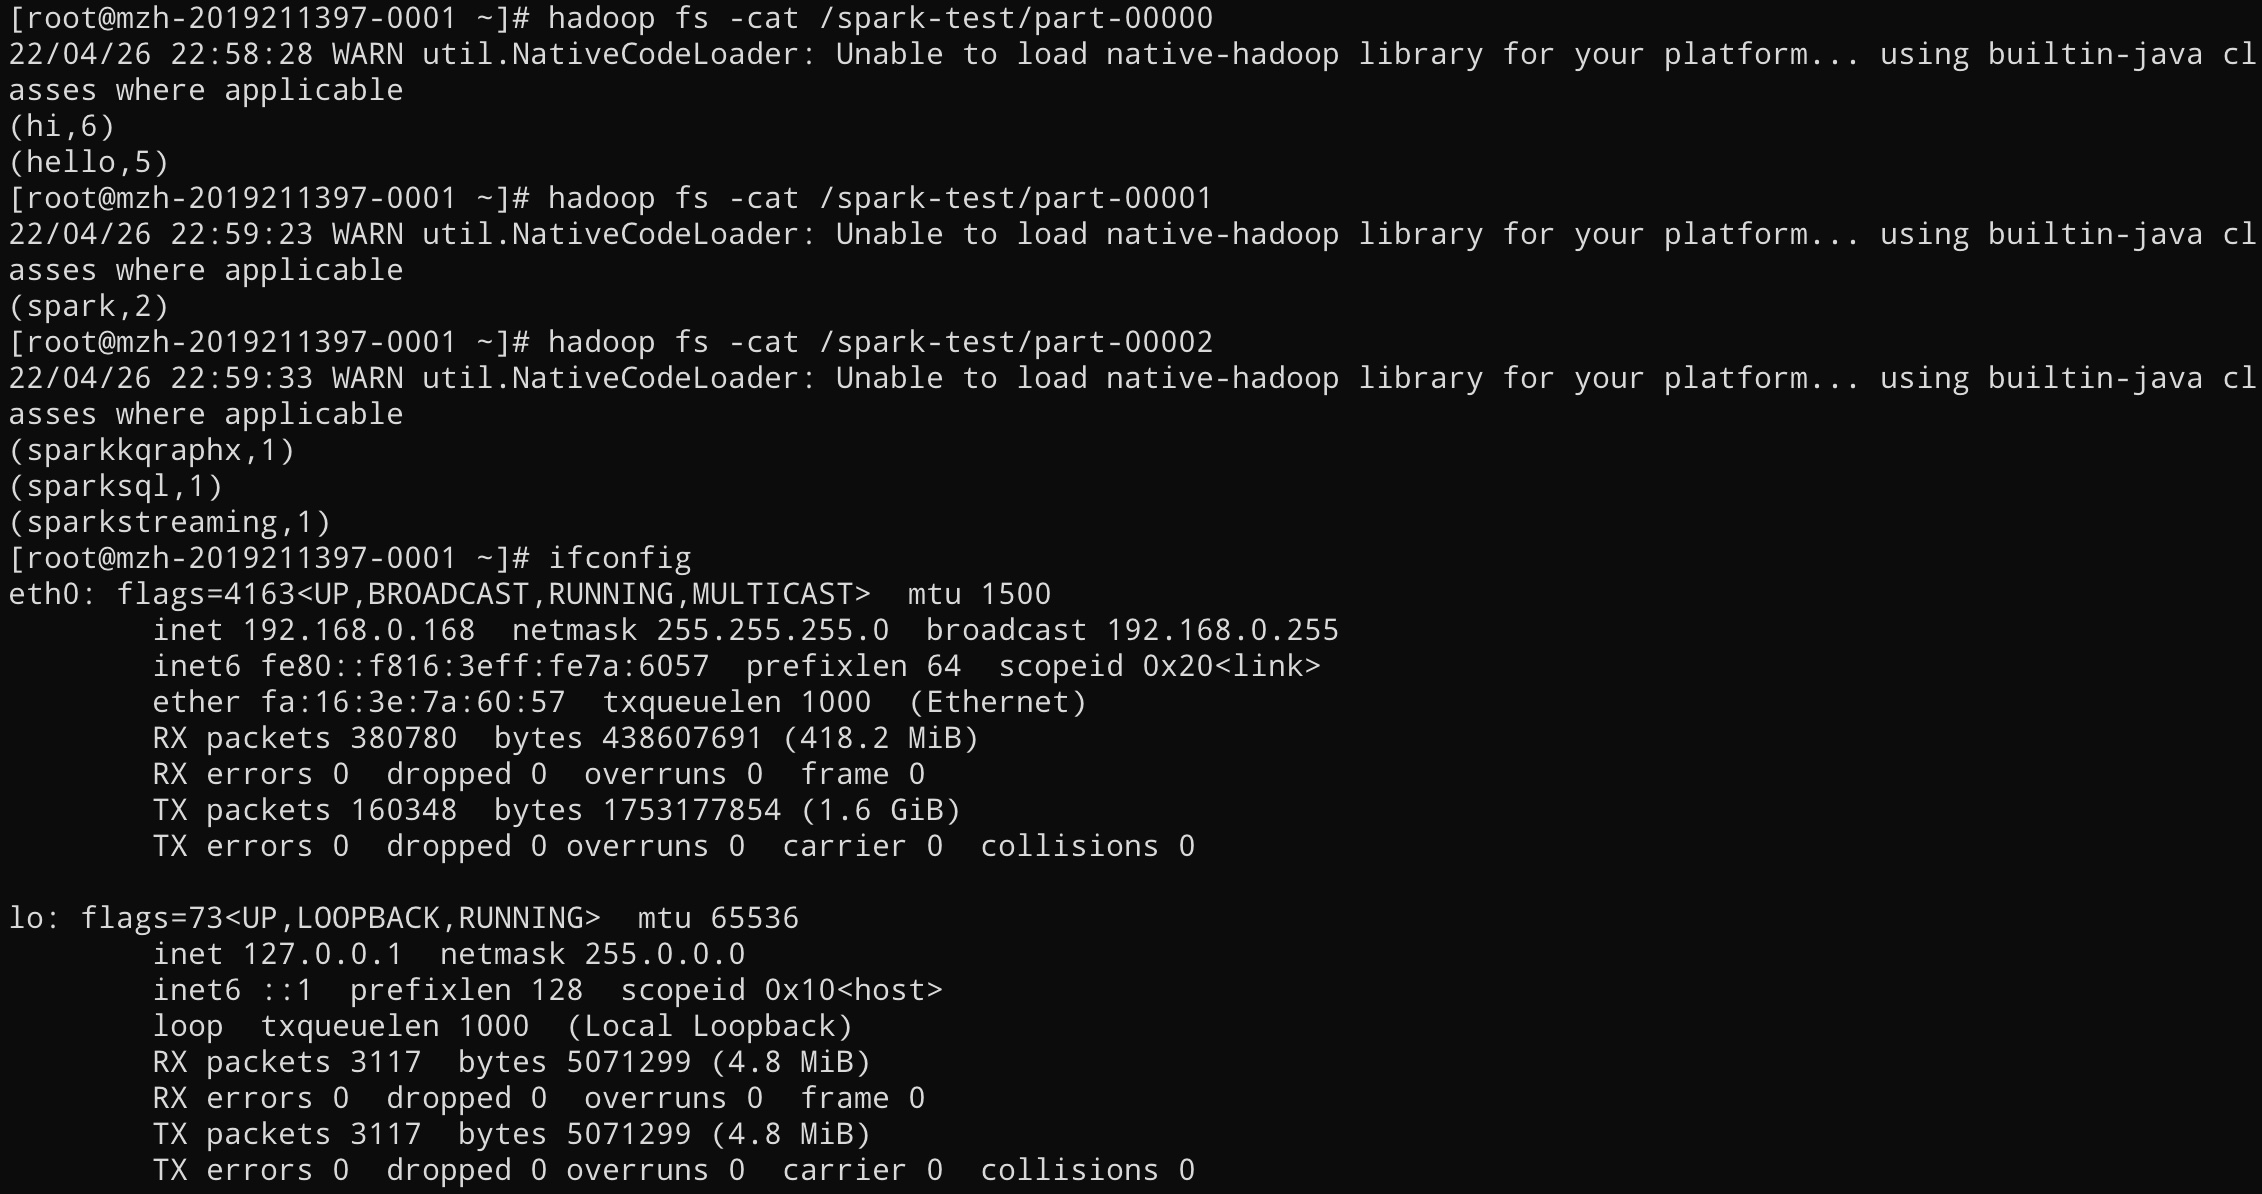
\includegraphics[width=\textwidth]{./images/res3.jpg}
    \caption{运行结果\label{fig:res3}}
\end{figure}

\paragraph{安装Hive}

安装 MySQL并启动MySQL Server的结果如\figref{fig:mysql1}。

\begin{figure}[!htb]
    \centering
    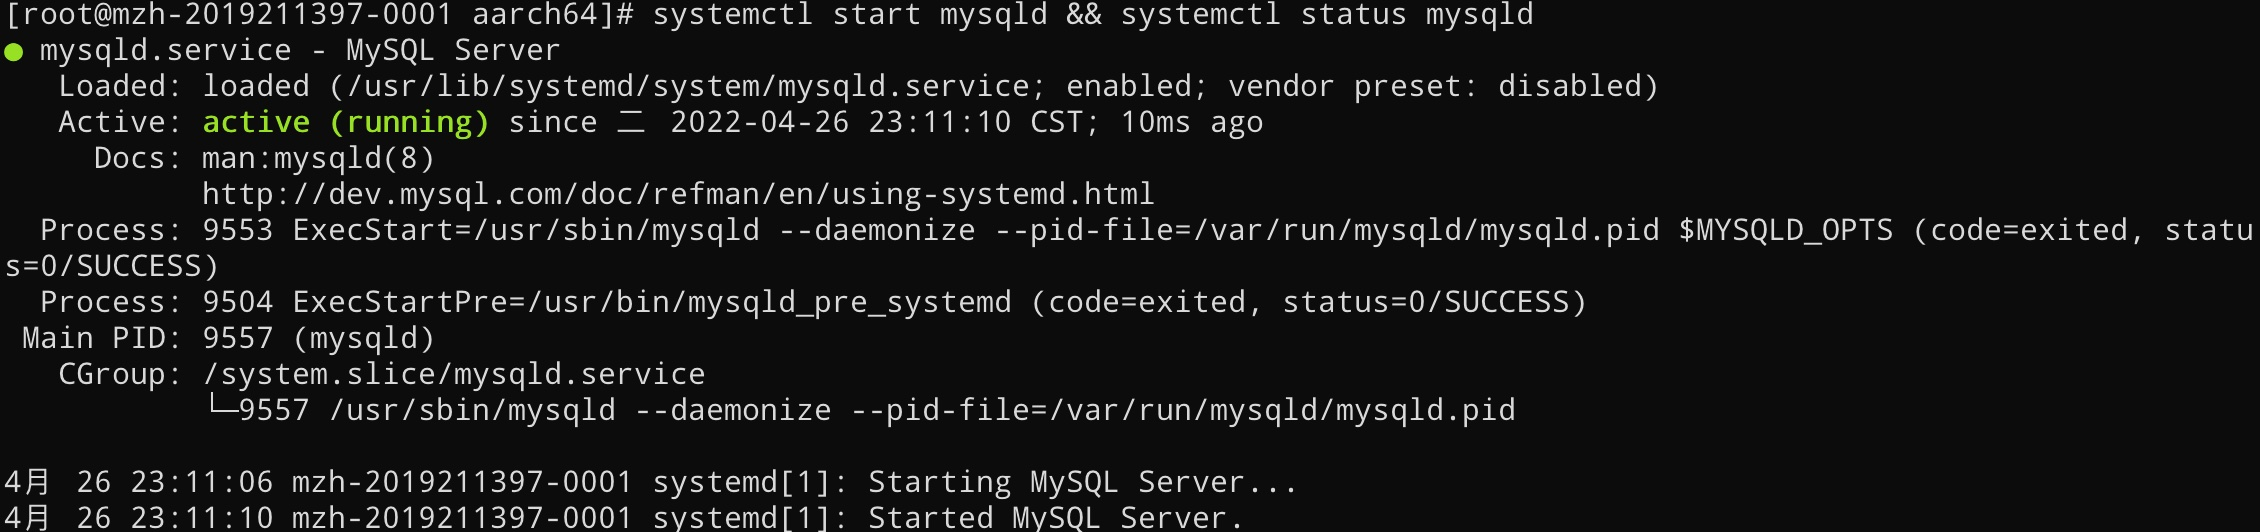
\includegraphics[width=\textwidth]{./images/mysql1.jpg}
    \caption{MySQL安装结果\label{fig:mysql1}}
\end{figure}

修改 MySQL root 密码、修改数据库默认编码的结果如\figref{fig:mysql2}。

\begin{figure}[!htb]
    \centering
    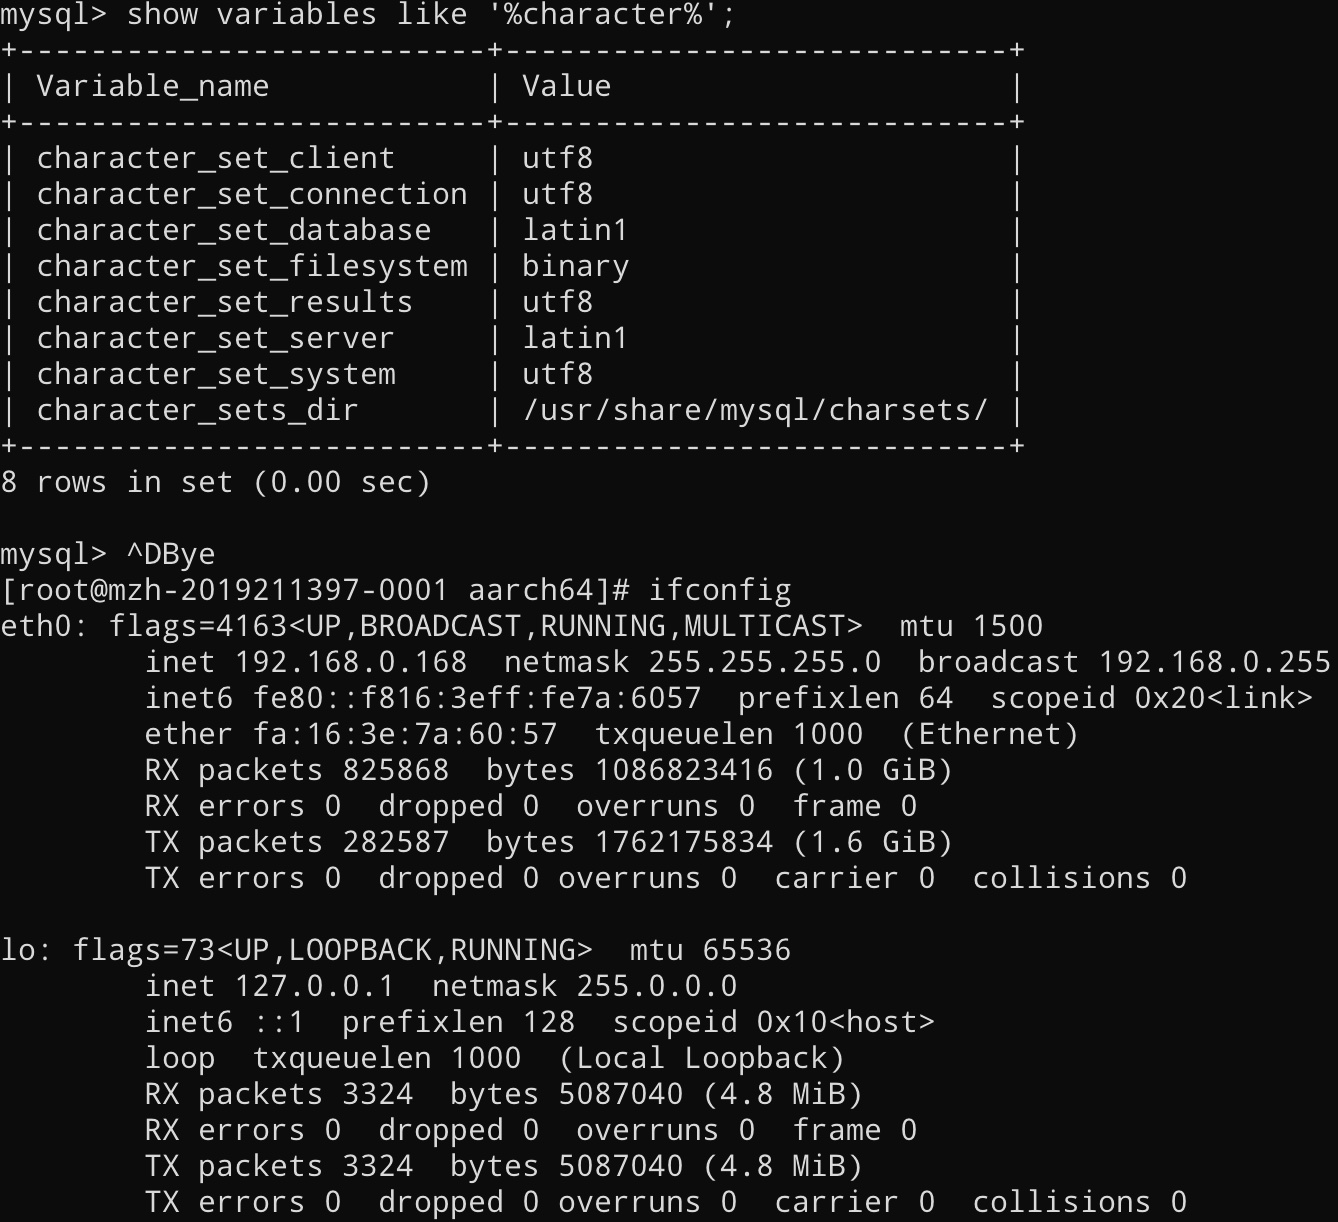
\includegraphics[width=0.7\textwidth]{./images/mysql2.jpg}
    \caption{MySQL修改编码结果\label{fig:mysql2}}
\end{figure}

\paragraph{Hive建库并导入数据}

在Hive中建立名为\mintinline{text}{spark}的数据库,其中创建名为\mintinline{text}{wordcount}的表,内容为一个文本文件的各个行,命令的运行结果如\figref{fig:hive}。

\begin{figure}[!htb]
    \centering
    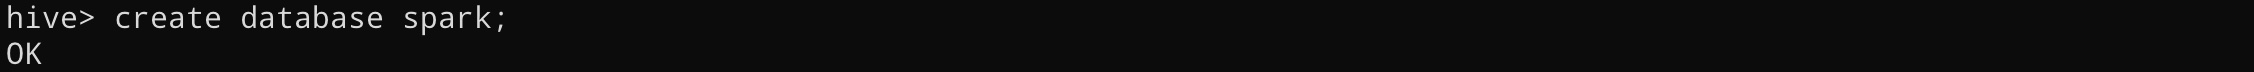
\includegraphics[width=\linewidth]{./images/hive1.jpg}
    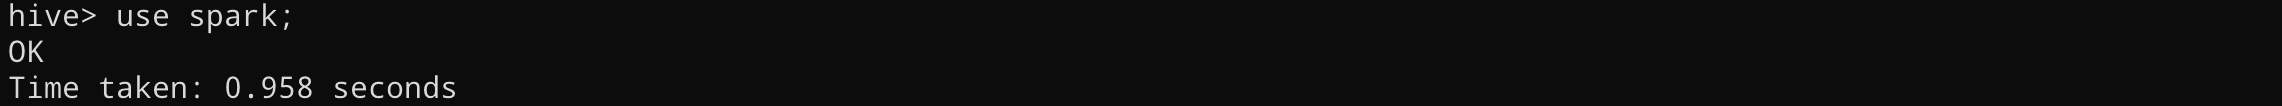
\includegraphics[width=\linewidth]{./images/hive2.jpg}
    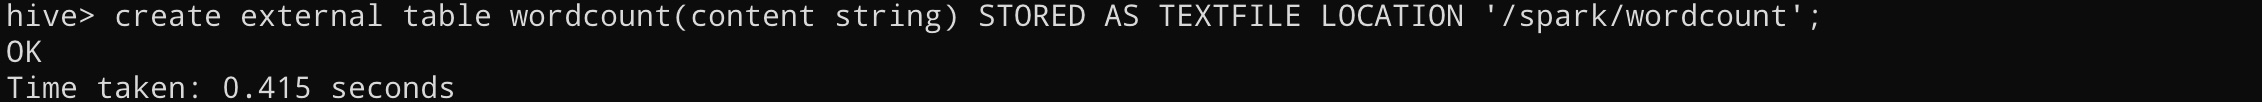
\includegraphics[width=\linewidth]{./images/hive3.jpg}
    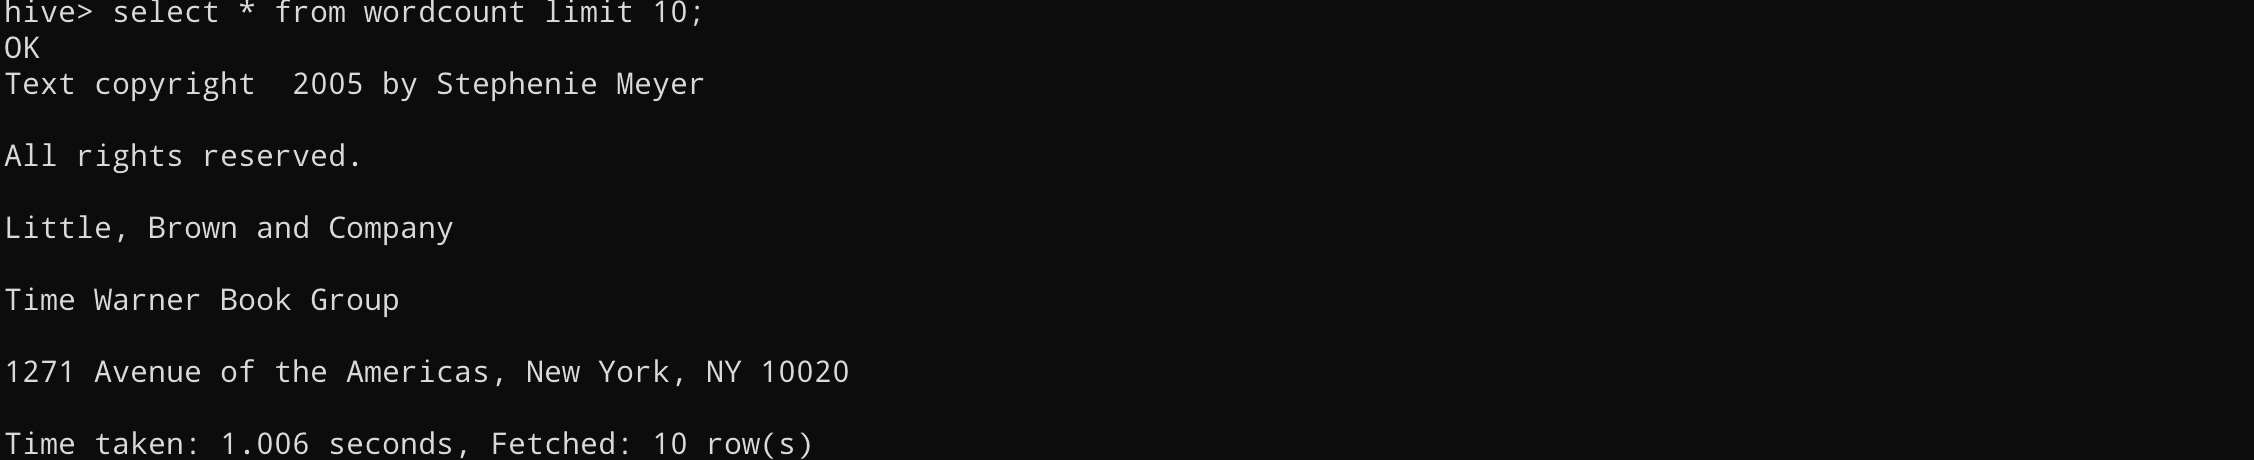
\includegraphics[width=\linewidth]{./images/hive4.jpg}
    \caption{Hive命令行运行结果\label{fig:hive}}
\end{figure}

编写程序如\figref{fig:code2}。

\begin{figure}[!htb]
    \centering
    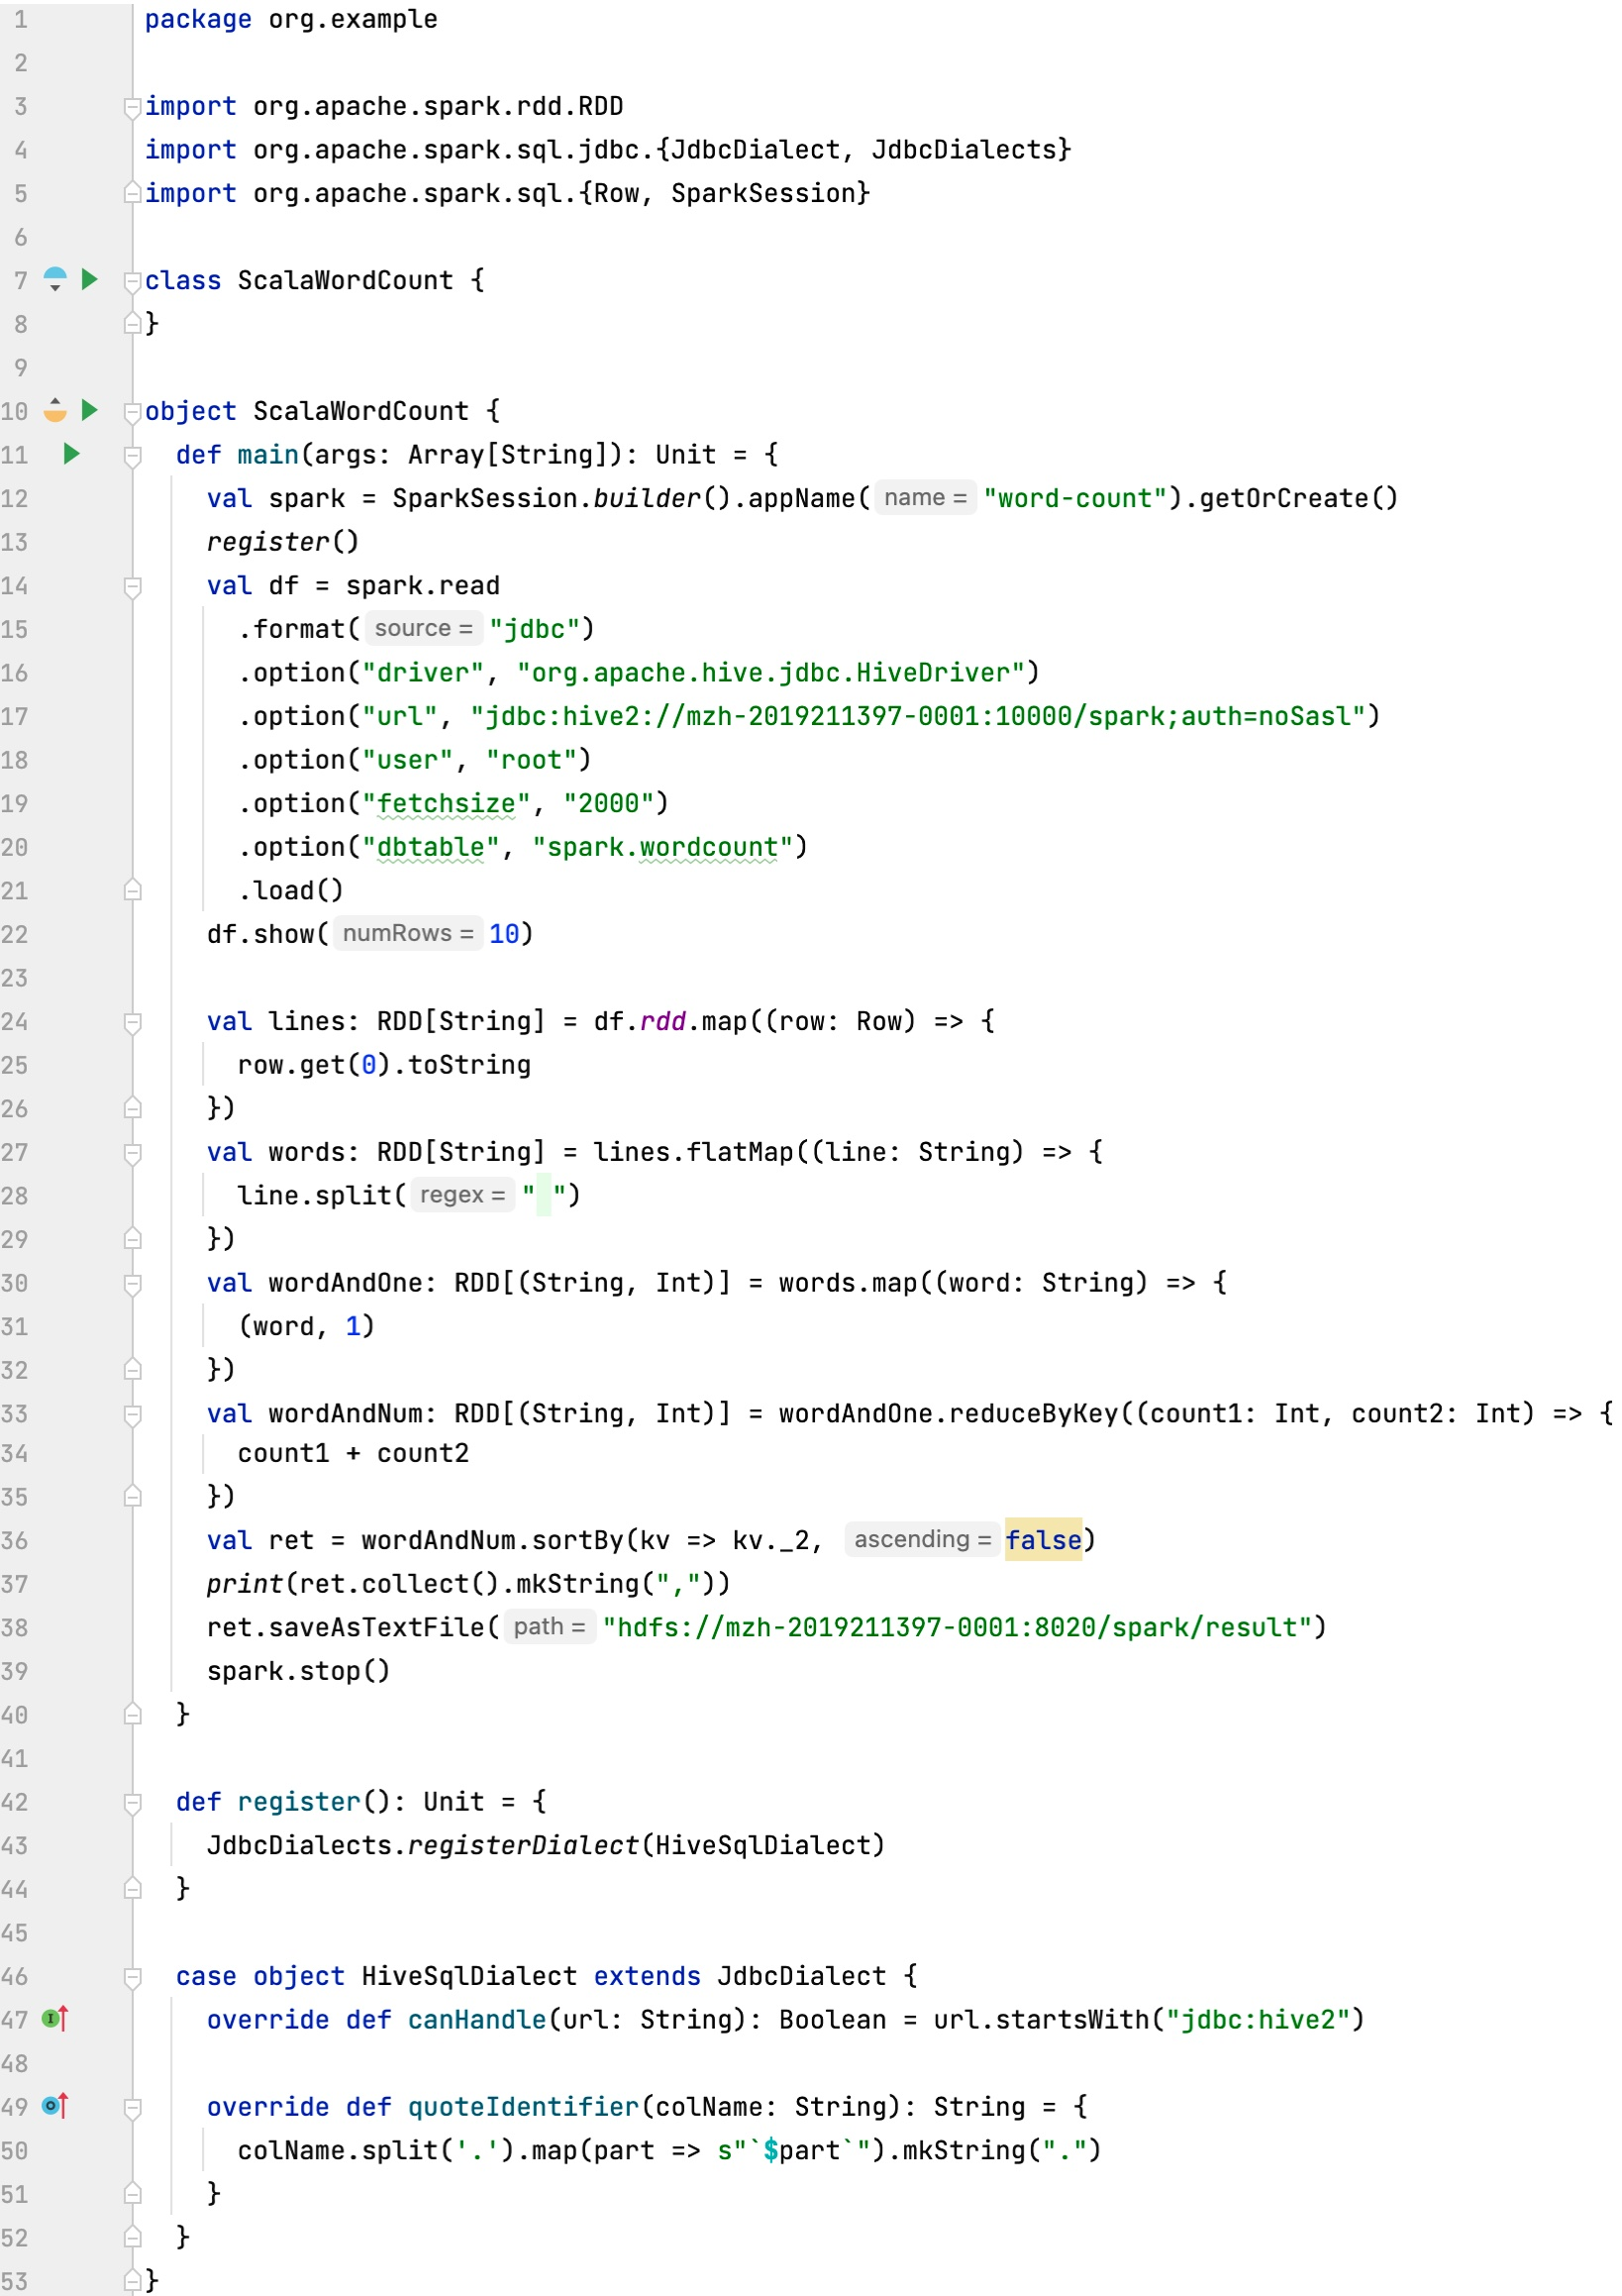
\includegraphics[width=0.7\textwidth]{./images/code2.jpg}
    \caption{wordcount程序\label{fig:code2}}
\end{figure}

相比于\figref{fig:code1},程序中将输入源改为Hive SQL Driver。

运行过程如\figref{fig:res4}。

\begin{figure}[!htb]
    \centering
    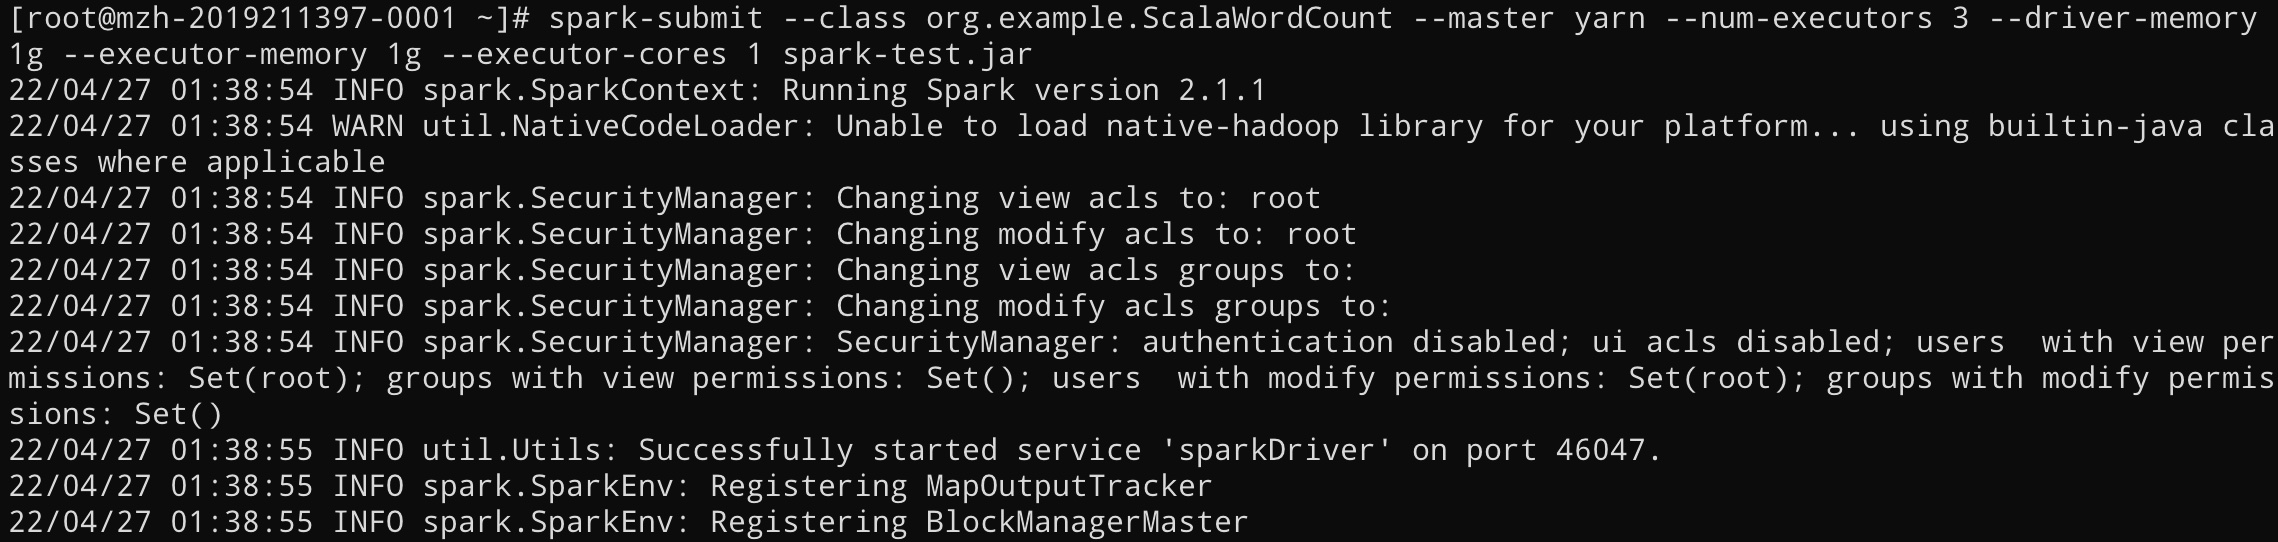
\includegraphics[width=\textwidth]{./images/res4.jpg}
    \caption{运行过程\label{fig:res4}}
\end{figure}

运行结果导出后显示前十行,如\figref{fig:res5}。

\begin{figure}[!htb]
    \centering
    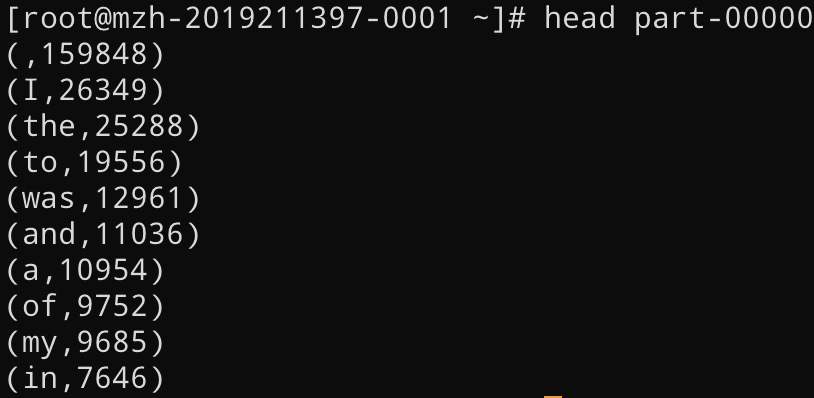
\includegraphics[width=0.5\textwidth]{./images/res5.jpg}
    \caption{运行结果\label{fig:res5}}
\end{figure}

\section{实验总结}

本次实验中我搭建了Spark和Hive环境,并且编写了Java代码实现了单词个数统计,在实验过程中我对Spark RDD的工作原理和Spark读取Hive的方式有了更深入的理解,我的Java编程水平也得到了提高,我从中受益良多。

\end{document}
